\documentclass[10pt, landscape, twocolumn]{article}

\usepackage[margin=0.5in, columnsep=0.4in]{geometry}
\usepackage{amsmath, amssymb, amsthm}
\usepackage{xcolor}
\usepackage{tabularx}
\usepackage{array}
\usepackage{tikz}
\usetikzlibrary{arrows.meta, positioning, calc, angles, quotes, shapes.geometric, 3d}
\usepackage{pgfplots}

\definecolor{themeblue}{RGB}{0, 90, 160}
\definecolor{themegray}{RGB}{80, 80, 80}

\pgfplotsset{compat=1.18}
\pgfplotsset{
  colormap={theme}{color(0)=(white) color(1)=(themeblue)},
  quadric axes/.style={
    width=\linewidth,
    height=3.1cm,
    hide axis,
    view={35}{30},
    colormap name=theme
  },
  quadric surf/.style={
    surf,
    z buffer=sort,
    samples=10,
    samples y=10,
    faceted color=themeblue!80!black,
    very thin
  }
}
\usepackage{enumitem}
\usepackage{mathpazo}
\usepackage{booktabs}

\pagestyle{empty}
\setlength{\parindent}{0pt}
\setlength{\parskip}{2pt}

\AtBeginDocument{
  \setlength{\abovedisplayskip}{3pt}
  \setlength{\belowdisplayskip}{3pt}
  \setlength{\abovedisplayshortskip}{1pt}
  \setlength{\belowdisplayshortskip}{1pt}
}

\newcommand{\cheatsheetsection}[1]{
    \vspace{0.6em}
    {\color{themeblue}\large\bfseries #1} \par
    \vspace{-0.5em}
    {\color{themeblue}\rule{\linewidth}{1pt}} \par
    \vspace{0.2em}
}

\newcommand{\cheatsheetsubsection}[1]{
    \vspace{0.4em}
    {\color{themeblue}\normalsize\bfseries #1} \par
    \vspace{0.1em}
}

\begin{document}

\begin{center}
    \vspace{-1em}
    {\color{themeblue}\huge\bfseries Formulario de Geometría Analítica}\\[0.1em]
    {\color{themegray}\small Formulario para Geometría Coordenada en 2D y 3D}\\[0.4em]
    {\color{themegray}\footnotesize \textbf{Por Roberto León Landeros}}
\end{center}
\vspace{-1em}

\cheatsheetsection{1. Fundamentos del Plano Cartesiano 2D}

\cheatsheetsubsection{Conceptos Básicos}
Dados los puntos $P_1(x_1, y_1)$ y $P_2(x_2, y_2)$:
\begin{itemize}[leftmargin=*, nosep]
    \item \textbf{Distancia:} $d = \sqrt{(x_2 - x_1)^2 + (y_2 - y_1)^2}$
    \item \textbf{Punto medio:} $M = \left( \frac{x_1 + x_2}{2}, \frac{y_1 + y_2}{2} \right)$
    \item \textbf{División en una razón $r$:} $P = \left( \frac{x_1 + rx_2}{1 + r}, \frac{y_1 + ry_2}{1 + r} \right)$
    \item \textbf{Baricentro (Centroide):} $G = \left( \frac{x_1+x_2+x_3}{3}, \frac{y_1+y_2+y_3}{3} \right)$
\end{itemize}

\textbf{Fórmula de la Lazada (Área de un polígono):}
\[ A = \frac{1}{2} \left| \sum_{i=1}^{n-1} (x_i y_{i+1} - x_{i+1} y_i) + (x_n y_1 - x_1 y_n) \right| \]

\cheatsheetsubsection{La Línea Recta}
\textbf{Pendiente ($m$):} $m = \frac{y_2 - y_1}{x_2 - x_1} = \tan \alpha$
\begin{itemize}[leftmargin=*, nosep]
    \item \textbf{Punto-pendiente:} $y - y_1 = m(x - x_1)$
    \item \textbf{Pendiente-ordenada al origen:} $y = mx + b$
    \item \textbf{Forma general:} $Ax + By + C = 0$
    \item \textbf{Forma simétrica:} \frac{x}{a} + \frac{y}{b} = 1
\end{itemize}
\textbf{Condiciones:} Paralelismo ($m_1 = m_2$), Perpendicularidad ($m_1 m_2 = -1$).

\textbf{Ángulo entre dos rectas:} $\tan \theta = \left| \frac{m_2 - m_1}{1 + m_1 m_2} \right|$

\textbf{Haz de rectas:} Rectas que pasan por la intersección de $L_1=0$ y $L_2=0$: $L_1 + kL_2 = 0$

\textbf{Distancia de un punto $P(x_0, y_0)$ a una recta:} $d = \frac{|Ax_0 + By_0 + C|}{\sqrt{A^2 + B^2}}$

\textbf{Distancia entre rectas paralelas:} $d = \frac{|C_2 - C_1|}{\sqrt{A^2 + B^2}}$

\vspace{-0.5em}
\begin{center}
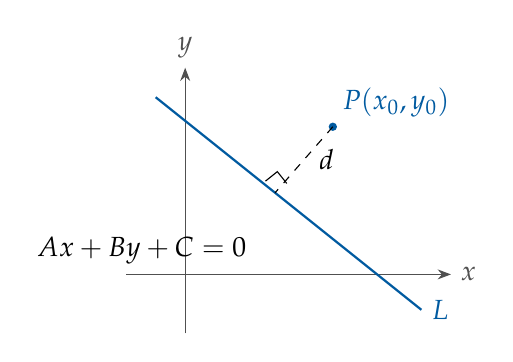
\begin{tikzpicture}[scale=0.75, >=Stealth]
    \draw[->, themegray] (-1,0) -- (4.5,0) node[right] {$x$};
    \draw[->, themegray] (0,-1) -- (0,3.5) node[above] {$y$};
    \draw[thick, themeblue] (-0.5, 3) -- (4, -0.6) node[right] {$L$};
    \fill[themeblue] (2.5, 2.5) circle (2pt) node[above right] {$P(x_0, y_0)$};
    \draw[dashed] (2.5, 2.5) -- (1.52, 1.38) node[midway, right=2pt] {$d$};
    \draw (1.52, 1.38) + (0.2, 0.16) -- + (0.04, 0.36) -- + (-0.16, 0.2);
    \node[anchor=north east] at (1.2, 0.8) {$Ax+By+C=0$};
\end{tikzpicture}
\end{center}
\vspace{-0.5em}

\cheatsheetsection{2. Secciones Cónicas}

\textbf{Ecuación general de 2do grado:} $Ax^2 + Bxy + Cy^2 + Dx + Ey + F = 0$

\textbf{Discriminante} $\Delta = B^2 - 4AC$:
\begin{itemize}[leftmargin=*, nosep]
    \item $\Delta < 0$: Elipse (Circunferencia si $A=C, B=0$)
    \item $\Delta = 0$: Parábola
    \item $\Delta > 0$: Hipérbola
\end{itemize}

\cheatsheetsubsection{Circunferencia y Parábola}
\textbf{Circunferencia:} Centro $(h,k)$, radio $r$: $(x-h)^2 + (y-k)^2 = r^2$

\textbf{Potencia de un punto $P(x_0, y_0)$ respecto a una circunferencia:} $p = (x_0-h)^2 + (y_0-k)^2 - r^2$ 
($p>0$: exterior, $p=0$: sobre la circunferencia, $p<0$: interior).

\textbf{Recta tangente a la circunferencia en $(x_1, y_1)$:} $(x_1-h)(x-h) + (y_1-k)(y-k) = r^2$

\vspace{-0.5em}
\begin{center}
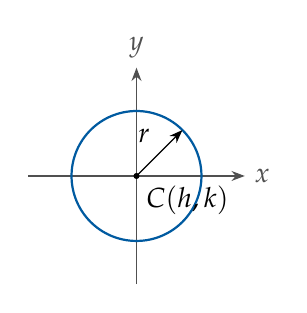
\begin{tikzpicture}[scale=0.55, >=Stealth]
    \draw[->, themegray] (-2.5,0) -- (2.5,0) node[right] {$x$};
    \draw[->, themegray] (0,-2.5) -- (0,2.5) node[above] {$y$};
    \draw[thick, themeblue] (0,0) circle (1.5cm);
    \fill (0,0) circle (2pt) node[below right] {$C(h,k)$};
    \draw[->] (0,0) -- (1.06, 1.06) node[midway, above left] {$r$};
\end{tikzpicture}
\end{center}
\vspace{-0.5em}

\textbf{Parábola} (Eje vertical): $(x-h)^2 = 4p(y-k)$
Vértice $V(h,k)$, Foco $F(h, k+p)$, Directriz $y = k-p$. Lado Recto $= |4p|$.

\textbf{Recta tangente a la parábola en $(x_1, y_1)$:} $(x_1-h)(x-h) = 2p(y+y_1-2k)$

\vspace{-0.5em}
\begin{center}
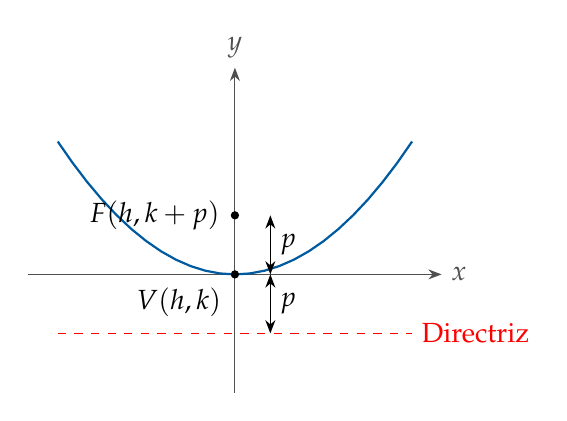
\begin{tikzpicture}[scale=0.75, >=Stealth]
    \draw[->, themegray] (-3.5,0) -- (3.5,0) node[right] {$x$};
    \draw[->, themegray] (0,-2) -- (0,3.5) node[above] {$y$};
    \draw[thick, themeblue, domain=-3:3] plot (\x, {0.25*\x*\x});
    \fill (0, 0) circle (2pt) node[below left=2pt] {$V(h,k)$};
    \fill (0, 1) circle (2pt) node[left=2pt] {$F(h,k+p)$};
    \draw[dashed, red] (-3, -1) -- (3, -1) node[right] {Directriz};
    \draw[<->] (0.6, 0) -- (0.6, 1) node[midway, right] {$p$};
    \draw[<->] (0.6, 0) -- (0.6, -1) node[midway, right] {$p$};
\end{tikzpicture}
\end{center}
\vspace{-0.5em}

\cheatsheetsubsection{Elipse e Hipérbola}
\textbf{Elipse} (Horizontal): $\frac{(x-h)^2}{a^2} + \frac{(y-k)^2}{b^2} = 1$
Focos $c^2 = a^2 - b^2$, Excentricidad $e = \frac{c}{a} < 1$.

\textbf{Lado Recto (Elipse e Hipérbola):} $LR = \frac{2b^2}{a}$

\textbf{Directrices (Elipse e Hipérbola):} $x = h \pm \frac{a}{e}$

\textbf{Recta tangente en $(x_1, y_1)$ (Regla del desdoblamiento):} $\frac{(x_1-h)(x-h)}{a^2} \pm \frac{(y_1-k)(y-k)}{b^2} = 1$ (+ para Elipse, - para Hipérbola)

\vspace{-0.5em}
\begin{center}
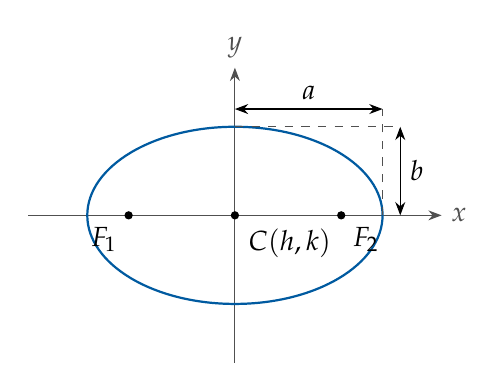
\begin{tikzpicture}[scale=0.75, >=Stealth]
    \draw[->, themegray] (-3.5,0) -- (3.5,0) node[right] {$x$};
    \draw[->, themegray] (0,-2.5) -- (0,2.5) node[above] {$y$};
    \draw[thick, themeblue] (0,0) ellipse (2.5cm and 1.5cm);
    \fill (-1.8, 0) circle (2pt) node[below left=1pt] {$F_1$};
    \fill (1.8, 0) circle (2pt) node[below right=1pt] {$F_2$};
    \fill (0,0) circle (2pt) node[below right=2pt] {$C(h,k)$};
    \draw[<->] (0, 1.8) -- (2.5, 1.8) node[midway, above] {$a$};
    \draw[<->] (2.8, 0) -- (2.8, 1.5) node[midway, right] {$b$};
    \draw[dashed, themegray] (2.5, 0) -- (2.5, 1.8);
    \draw[dashed, themegray] (0, 1.5) -- (2.8, 1.5);
\end{tikzpicture}
\end{center}
\vspace{-0.5em}

\textbf{Hipérbola} (Horizontal): $\frac{(x-h)^2}{a^2} - \frac{(y-k)^2}{b^2} = 1$
Focos $c^2 = a^2 + b^2$, Asíntotas $y - k = \pm \frac{b}{a}(x - h)$.

\vspace{-0.5em}
\begin{center}
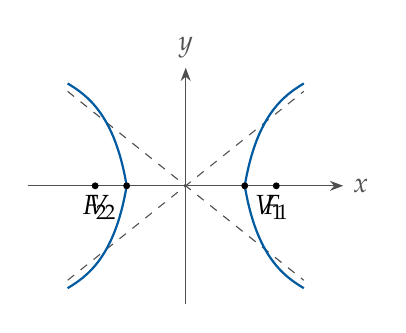
\begin{tikzpicture}[scale=0.5, >=Stealth]
    \draw[->, themegray] (-4,0) -- (4,0) node[right] {$x$};
    \draw[->, themegray] (0,-3) -- (0,3) node[above] {$y$};
    \draw[dashed, themegray] (-3,-2.4) -- (3,2.4);
    \draw[dashed, themegray] (-3,2.4) -- (3,-2.4);
    \draw[thick, themeblue] (1.5,0) .. controls (1.8, 1.8) and (2.5, 2.3) .. (3, 2.6);
    \draw[thick, themeblue] (1.5,0) .. controls (1.8, -1.8) and (2.5, -2.3) .. (3, -2.6);
    \draw[thick, themeblue] (-1.5,0) .. controls (-1.8, 1.8) and (-2.5, 2.3) .. (-3, 2.6);
    \draw[thick, themeblue] (-1.5,0) .. controls (-1.8, -1.8) and (-2.5, -2.3) .. (-3, -2.6);
    \fill (1.5,0) circle (2.5pt) node[below right] {$V_1$};
    \fill (-1.5,0) circle (2.5pt) node[below left] {$V_2$};
    \fill (2.3,0) circle (2.5pt) node[below] {$F_1$};
    \fill (-2.3,0) circle (2.5pt) node[below] {$F_2$};
\end{tikzpicture}
\end{center}
\vspace{-0.5em}

\cheatsheetsubsection{Transformaciones y Cónicas Polares}
\textbf{Rotación de ejes:} Para eliminar el término $xy$, rotar un ángulo $\theta$:
\[ \tan(2\theta) = \frac{B}{A - C} \]
Ecuaciones: $x = x'\cos\theta - y'\sin\theta$, $y = x'\sin\theta + y'\cos\theta$

\textbf{Ecuación polar universal:} $r = \frac{ed}{1 \pm e \cos\theta}$ ($e$: excentricidad, $d$: distancia a la directriz).

\cheatsheetsection{3. Coordenadas Polares y Paramétricas}
\textbf{Conversión $\mathbb{R}^2 \leftrightarrow$ Polar:}
$x = r \cos\theta, \quad y = r \sin\theta, \quad r^2 = x^2 + y^2, \quad \tan\theta = \frac{y}{x}$

\vspace{-0.5em}
\begin{center}
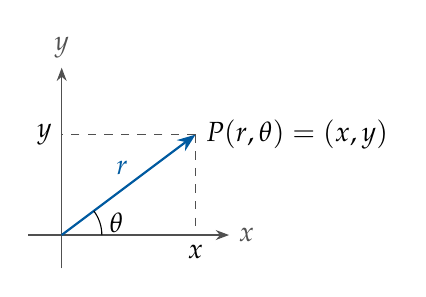
\begin{tikzpicture}[scale=0.85, >=Stealth]
    \draw[->, themegray] (-0.5,0) -- (2.5,0) node[right] {$x$};
    \draw[->, themegray] (0,-0.5) -- (0,2.5) node[above] {$y$};
    \draw[thick, themeblue, ->] (0,0) -- (2,1.5) node[right, text=black] {$P(r,\theta) = (x,y)$};
    \draw[dashed, themegray] (2,1.5) -- (2,0) node[below, text=black] {$x$};
    \draw[dashed, themegray] (2,1.5) -- (0,1.5) node[left, text=black] {$y$};
    \draw (0.6,0) arc (0:36.87:0.6) node[midway, right] {$\theta$};
    \node[themeblue] at (0.9, 1.0) {$r$};
\end{tikzpicture}
\end{center}
\vspace{-0.5em}

\textbf{Ecuaciones Paramétricas:} Representan variables mediante un parámetro $t$.
Circunferencia: $x = r\cos t, y = r\sin t$.
Cicloide: $x = R(t - \sin t), y = R(1 - \cos t)$.

\cheatsheetsection{4. Vectores ($\mathbb{R}^2, \mathbb{R}^3$)}
\textbf{Operaciones:} $\vec{u} \pm \vec{v} = \langle u_1 \pm v_1, u_2 \pm v_2, u_3 \pm v_3 \rangle$

\textbf{Producto escalar (Punto):} $\vec{u} \cdot \vec{v} = \|\vec{u}\|\|\vec{v}\|\cos\theta = u_1 v_1 + u_2 v_2 + u_3 v_3$

\textbf{Proyección vectorial:} $\text{proy}_{\vec{v}}\vec{u} = \left(\frac{\vec{u} \cdot \vec{v}}{\|\vec{v}\|^2}\right)\vec{v}$

\textbf{Producto vectorial (Cruz)} (Área del paralelogramo):
\[ \vec{u} \times \vec{v} = \begin{vmatrix} \hat{i} & \hat{j} & \hat{k} \\ u_1 & u_2 & u_3 \\ v_1 & v_2 & v_3 \end{vmatrix} \]
$\|\vec{u} \times \vec{v}\| = \|\vec{u}\| \|\vec{v}\| \sin \theta$

\vspace{-0.5em}
\begin{center}
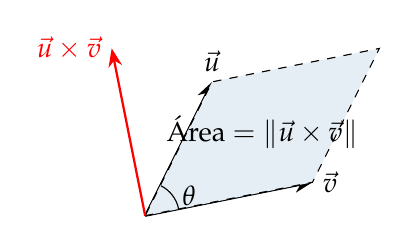
\begin{tikzpicture}[scale=0.85, >=Stealth]
    \draw[->, thick] (0,0) -- (2.5,0.5) node[right] {$\vec{v}$};
    \draw[->, thick] (0,0) -- (1,2) node[above] {$\vec{u}$};
    \draw[dashed, fill=themeblue!10] (0,0) -- (2.5,0.5) -- (3.5,2.5) -- (1,2) -- cycle;
    \draw[->, thick, red] (0,0) -- (-0.5, 2.5) node[left] {$\vec{u} \times \vec{v}$};
    \node at (1.75, 1.25) {Área $= \|\vec{u} \times \vec{v}\|$};
    \draw (0.5, 0.1) arc (11.3:63.4:0.5) node[midway, right] {$\theta$};
\end{tikzpicture}
\end{center}
\vspace{-0.5em}

\textbf{Producto triple escalar (Volumen del paralelepípedo):}
$V = |\vec{u} \cdot (\vec{v} \times \vec{w})|$

\textbf{Distancia de un punto a una recta en $\mathbb{R}^3$:}
$d = \frac{\|\vec{v} \times (\vec{P} - \vec{P_0})\|}{\|\vec{v}\|}$

\cheatsheetsection{5. Geometría Analítica en 3D}

\vspace{-0.5em}
\begin{center}
\begin{tikzpicture}[scale=0.9, >=Stealth, x={(-0.5cm,-0.4cm)}, y={(1cm,0cm)}, z={(0cm,1cm)}]
    \draw[->, themegray] (0,0,0) -- (2.5,0,0) node[below left] {$x$};
    \draw[->, themegray] (0,0,0) -- (0,2.5,0) node[right] {$y$};
    \draw[->, themegray] (0,0,0) -- (0,0,2.5) node[above] {$z$};
    \draw[->, thick, themeblue] (0,0,0) -- (1.5,2,1.8) node[right, text=black] {$P(x,y,z)$};
    \draw[dashed, themegray] (1.5,2,1.8) -- (1.5,2,0);
    \draw[dashed, themegray] (1.5,2,0) -- (1.5,0,0);
    \draw[dashed, themegray] (1.5,2,0) -- (0,2,0);
    \draw[dashed, themegray] (1.5,2,1.8) -- (0,0,1.8);
\end{tikzpicture}
\end{center}
\vspace{-0.5em}

\cheatsheetsubsection{La Recta en el Espacio}
Dado un punto $\vec{r_0}(x_0, y_0, z_0)$ y un vector director $\vec{v} = \langle v_x, v_y, v_z \rangle$:
\begin{itemize}[leftmargin=*, nosep]
    \item \textbf{Vectorial:} $\vec{r}(t) = \vec{r_0} + t\vec{v}$
    \item \textbf{Paramétrica:} $x = x_0 + tv_x, \quad y = y_0 + tv_y, \quad z = z_0 + tv_z$
    \item \textbf{Simétrica:} \frac{x-x_0}{v_x} = \frac{y-y_0}{v_y} = \frac{z-z_0}{v_z}
\end{itemize}

\textbf{Distancia entre rectas cruzadas:} Dadas $\vec{r_1}(t) = \vec{P_1} + t\vec{v_1}$ y $\vec{r_2}(t) = \vec{P_2} + t\vec{v_2}$:
\[ d = \frac{|(\vec{P_2} - \vec{P_1}) \cdot (\vec{v_1} \times \vec{v_2})|}{\|\vec{v_1} \times \vec{v_2}\|} \]

\cheatsheetsubsection{El Plano}
Dado un punto $\vec{r_0}$ y un vector normal $\vec{n} = \langle A, B, C \rangle$:
\begin{itemize}[leftmargin=*, nosep]
    \item \textbf{Forma normal:} $\vec{n} \cdot (\vec{r} - \vec{r_0}) = 0$
    \item \textbf{Forma general:} $Ax + By + Cz + D = 0$
    \item \textbf{Ángulo entre planos:} $\cos \theta = \frac{|\vec{n_1} \cdot \vec{n_2}|}{\|\vec{n_1}\| \|\vec{n_2}\|}$
\end{itemize}

\textbf{Ángulo entre una recta ($\vec{v}$) y un plano ($\vec{n}$):} $\sin \alpha = \frac{|\vec{v} \cdot \vec{n}|}{\|\vec{v}\| \|\vec{n}\|}$

\textbf{Distancia entre planos paralelos:} $d = \frac{|D_2 - D_1|}{\sqrt{A^2 + B^2 + C^2}}$

\textbf{Vector director de la recta de intersección de dos planos:} $\vec{v} = \vec{n_1} \times \vec{n_2}$

\vspace{-0.5em}
\begin{center}
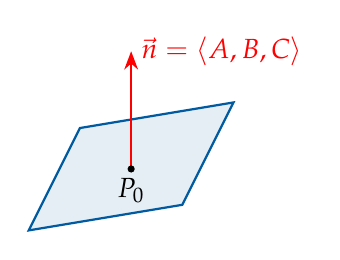
\begin{tikzpicture}[scale=0.65, >=Stealth]
    \filldraw[fill=themeblue!10, draw=themeblue, thick] (0,0) -- (3,0.5) -- (4,2.5) -- (1,2) -- cycle;
    \draw[->, thick, red] (2,1.2) -- (2,3.5) node[right] {$\vec{n} = \langle A, B, C \rangle$};
    \fill (2,1.2) circle (2pt) node[below] {$P_0$};
\end{tikzpicture}
\end{center}
\vspace{-0.5em}

\cheatsheetsubsection{Superficies Cuádricas}
\renewcommand{\arraystretch}{1.5}
\begin{tabular}{@{} >{\centering\arraybackslash}p{0.48\linewidth} >{\centering\arraybackslash}p{0.48\linewidth} @{}}
\textbf{Elipsoide} & \textbf{Paraboloide elíptico} \\
$\frac{x^2}{a^2} + \frac{y^2}{b^2} + \frac{z^2}{c^2} = 1$ & $z = \frac{x^2}{a^2} + \frac{y^2}{b^2}$ \\
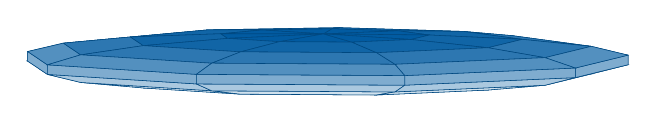
\begin{tikzpicture}
\begin{axis}[quadric axes]
\addplot3[quadric surf, domain=0:360, y domain=-90:90] ({2*cos(y)*cos(x)}, {1.5*cos(y)*sin(x)}, {sin(y)});
\end{axis}
\end{tikzpicture}
&
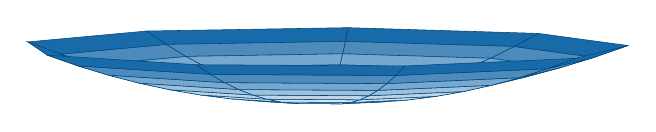
\begin{tikzpicture}
\begin{axis}[quadric axes]
\addplot3[quadric surf, domain=0:360, y domain=0:1.5] ({y*cos(x)}, {1.5*y*sin(x)}, {y^2});
\end{axis}
\end{tikzpicture} \\

\textbf{Paraboloide hiperbólico} & \textbf{Hiperboloide (1 hoja)} \\
$z = \frac{y^2}{b^2} - \frac{x^2}{a^2}$ & $\frac{x^2}{a^2} + \frac{y^2}{b^2} - \frac{z^2}{c^2} = 1$ \\
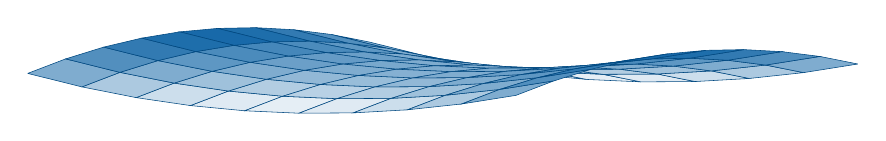
\begin{tikzpicture}
\begin{axis}[quadric axes]
\addplot3[quadric surf, domain=-1.5:1.5, y domain=-1.5:1.5] ({x}, {y}, {x^2 - y^2});
\end{axis}
\end{tikzpicture}
&
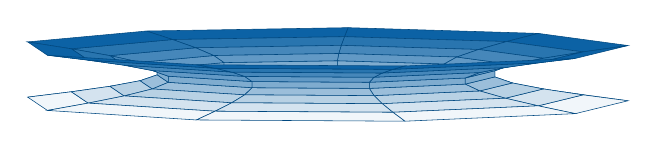
\begin{tikzpicture}
\begin{axis}[quadric axes]
\addplot3[quadric surf, domain=0:360, y domain=-1.5:1.5] ({sqrt(1+y^2)*cos(x)}, {1.5*sqrt(1+y^2)*sin(x)}, {y});
\end{axis}
\end{tikzpicture} \\

\textbf{Hiperboloide (2 hojas)} & \textbf{Cono elíptico} \\
$\frac{z^2}{c^2} - \frac{x^2}{a^2} - \frac{y^2}{b^2} = 1$ & $\frac{z^2}{c^2} = \frac{x^2}{a^2} + \frac{y^2}{b^2}$ \\
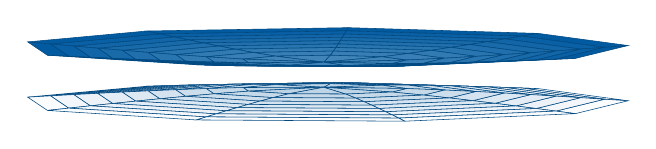
\begin{tikzpicture}
\begin{axis}[quadric axes]
\addplot3[quadric surf, domain=0:360, y domain=1:2.2] ({sqrt(y^2-1)*cos(x)}, {1.5*sqrt(y^2-1)*sin(x)}, {y});
\addplot3[quadric surf, domain=0:360, y domain=1:2.2] ({sqrt(y^2-1)*cos(x)}, {1.5*sqrt(y^2-1)*sin(x)}, {-y});
\end{axis}
\end{tikzpicture}
&
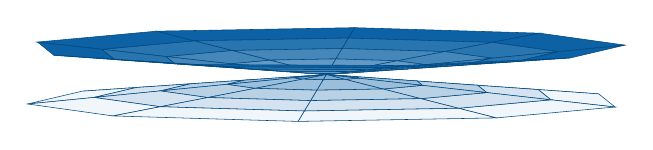
\begin{tikzpicture}
\begin{axis}[quadric axes]
\addplot3[quadric surf, domain=0:360, y domain=-2:2] ({y*cos(x)}, {1.5*y*sin(x)}, {y});
\end{axis}
\end{tikzpicture}
\end{tabular}

\newpage
\cheatsheetsection{6. Matrices y Transformaciones Lineales}

\cheatsheetsubsection{Transformaciones Geométricas}
Aplicadas mediante multiplicación de matrices $\vec{v}' = T \vec{v}$.

\vspace{-0.5em}
\begin{center}
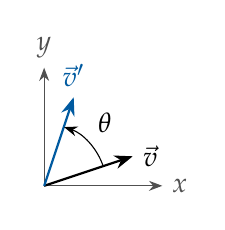
\begin{tikzpicture}[scale=0.75, >=Stealth]
    \draw[->, themegray] (0,0) -- (2,0) node[right] {$x$};
    \draw[->, themegray] (0,0) -- (0,2) node[above] {$y$};
    \draw[->, thick] (0,0) -- (1.5, 0.5) node[right] {$\vec{v}$};
    \draw[->, thick, themeblue] (0,0) -- (0.5, 1.5) node[above] {$\vec{v}'$};
    \draw[->] (1.0, 0.33) arc (18.4:71.5:1.05) node[midway, above right] {$\theta$};
\end{tikzpicture}
\end{center}
\vspace{-0.5em}

\textbf{Matriz de rotación (2D, antihoraria $\theta$):}
\[ R_\theta = \begin{bmatrix} \cos\theta & -\sin\theta \\ \sin\theta & \cos\theta \end{bmatrix} \]
\textbf{Matriz de escalamiento:} $S(s_x, s_y) = \begin{bmatrix} s_x & 0 \\ 0 & s_y \end{bmatrix}$

\textbf{Cambio de base (Diagonalización):}
Utilizado para alinear secciones cónicas rotadas a los ejes canónicos. $A = PDP^{-1}$

\cheatsheetsubsection{Coordenadas Homogéneas}
Expande los vectores de $\mathbb{R}^2$ a dimensiones de $3 \times 1$ para permitir traslaciones como multiplicaciones de matrices (transformaciones afines). Un punto 2D $(x,y)$ se convierte en $(x, y, 1)$.

\textbf{Matriz de traslación:}
\[ \begin{bmatrix} x' \\ y' \\ 1 \end{bmatrix} = \begin{bmatrix} 1 & 0 & t_x \\ 0 & 1 & t_y \\ 0 & 0 & 1 \end{bmatrix} \begin{bmatrix} x \\ y \\ 1 \end{bmatrix} = \begin{bmatrix} x + t_x \\ y + t_y \\ 1 \end{bmatrix} \]

\end{document}